\section{Безопасность и экологичность проекта}

В эпоху активного развития информационных и компьютерных технологий возникает проблема сохранения благополучия и здоровья человека.
Из-за увеличения продолжительности непрерывной работы за персональной ЭВМ, а также последствий этого, будь то постоянный шум, сидячий режим работы или излишняя нагрузка на органы зрения, начали более активное развитие некоторые заболевания и отклонения в здоровье человека.

В отрасли информационных технологий охрана труда в последнее время получает всё большее внимание со стороны работодателей, так как увеличивается число случаев профессиональных заболеваний программистов ввиду особенностей их деятельности.
Это в свою очередь негативно сказывается на производительности работника.

Также о повышенном внимании к безопасности при работе с персональной ЭВМ можно судить по тому, что уже на протяжении нескольких лет студенты, обучающиеся на направлениях, связанных с компьютерными науками, не только разрабатывают программные продукты, но и описывают и расчитывают условия безопасной работы за ПЭВМ.

\subsection{Исходные данные}

\begin{footnotesize}
\begin{longtable}[h]{|p{0.05\textwidth}|p{0.35\textwidth}|p{0.5\textwidth}|}
	\caption{\label{tab:ecol-source}Исходные данные для проектирования} \\
	\hline
		\textbf{№№} &
		\textbf{Данные} &
		\textbf{Название} \\
	\hline \endfirsthead
	\caption*{\raggedleft Продолжение таблицы \ref{tab:ecol-source}}\\
	\hline
		\textbf{№№} &
		\textbf{Данные} &
		\textbf{Название} \\
	\hline \endhead
		1 & 
		Тема дипломного проекта &
		\WorkName \\
	\hline
		2 & 
		Технологический процесс &
		Единичный технологический процесс \\
	\hline
		3 & 
		Оборудование, в т. ч. паспортные данные &
		\begin{enumerate}
			\item Ноутбук Samsung NP350E5C-S06RU 
			\item Маршрутизатор NetGear WNR3500L v2
		\end{enumerate} \\
	\hline
		4 & 
		Персонал (состав, профессии) &
		1 программист, 1 сотрудник отдела контроля качества \\
	\hline
		5 & 
		Исходное состояние системы, ресурсы, материалы &
		Ресурсами является Интернет и доступ к внутренней сети ООО <<АИС Город>>.
		Материалами являются внутренние регламенты ООО <<АИС Город>>.\\
	\hline
		6 & 
		Энергоносители (электричество, вода, пар, газ, уголь) и их характеристики &
		Бытовая электросеть 220В. \\
	\hline
		7 & 
		Расположение рабочего места, функции персонала &
		Рабочее место программиста располагается в ФГБОУ ВПО УлГТУ.
		Программист разрабатывает ИС. \newline
		Рабочее место сотрудника отдела контроля качества располагается в офисе ООО АИС Город.
		Сотрудник отдела КК следит за соблюдением технического задания при разработке ИС. \\
	\hline
		8 & 
		Признаки отнесения объекта к опасным промышленным объектам &
		Отсутствуют. \\
	\hline
		9 & 
		Санитарная характеристика производства &
		Отсутствует. \\
	\hline
		10 & 
		Характеристика помещений по электроопасности &
		Помещения без повышенной опасности. \\
	\hline
		11 & 
		Характеристика среды помещений &
		Сухие помещения. \\
	\hline
		12 & 
		Категория производства по взрывопожарной опасности &
		Д --- пониженная пожароопасность. \\
	\hline
		13 & 
		Класс пожароопасной зоны &
		Отсутствует. \\
	\hline
		14 & 
		Класс взрывоопасной зоны &
		Отсутствует. \\
	\hline
		15 & 
		Рассматриваемые стадии <<жизненного цикла>> продукции &
		\begin{enumerate}
			\item Формирование требований
			\item Разработка концепции АС 
			\item Техническое задание 
			\item Эскизный проект
			\item Технический проект
			\item Рабочая документация
			\item Тестирование
			\item Ввод в действие
			\item Сопровождение
		\end{enumerate} \\
	\hline
\end{longtable}
\begin{longtable}[h]{|p{0.05\textwidth}|p{0.35\textwidth}|p{0.5\textwidth}|}
	\caption*{\raggedleft Окончание таблицы \ref{tab:ecol-source}}\\
	\hline
		\textbf{№№} &
		\textbf{Данные} &
		\textbf{Название} \\
	\hline \endhead
	\hline
		16 & 
		Классы условий труда в соответствии с Картой аттестации рабочего места по условиям труда: \newline
		по вредности, \newline
		по травмоопасности &
		По вредности --- вредный (III) класс. \newline
		По травмоопасности --- допустимый (II) класс. \\
	\hline
		17 & 
		Виды загрязнений окружающей среды &
		Отсутствуют. \\
	\hline
\end{longtable}
\end{footnotesize}

~

\subsection{Перечень нормативных документов}

\begin{enumerate}[1.]
	\item Санитарные правила и нормы. СанПиН 2.2.2./2.4.1340-03 Гигиенические требования к персональным электронно-вычислительным машинам и организации работы. 
	\item <<Руководство по гигиенической оценке факторов рабочей среды  и трудовых процессов. Критерии и классификация условий труда>>. Р 2.2.2006-05.
	\item ГОСТ 12.0.003-74.ССБТ. (СТ СЭВ 790-77) Опасные и вредные производственные факторы. Классификация. М.: Изд-во стандартов, 1996.
	\item ГОСТ 12.1.003-83.ССБТ. Шум. Общие требования безопасности. М.: Изд-во стандартов.1996.
	\item ГОСТ 12.1.004-91.ССБТ. Пожарная безопасность. Общие требования. М.: Изд-во стандартов, 1996.
	\item ГОСТ 12.1.005-88.ССБТ. Общие санитарно-гигиенические требования к воздуху рабочей зоны. М.: Изд-во стандартов, 1996.
	\item ГОСТ 12.1.006-88.ССБТ. Электромагнитные поля  радиочастот. Допустимые уровни на рабочих местах и требования к проведения контроля. М.: Изд-во стандартов, 1998.
	\item ГОСТ 12.1.019-79.ССБТ (СТ СЭВ 4880-84). Электробезопасность. Общие требования. М.: Изд-во стандартов, 1996.
	\item ГОСТ 12.1.030-81.ССБТ. Электробезопасность. Защитное заземление зануление. М.: Изд-во стандартов, 1996.
	\item ГОСТ 12.1.038-82.ССБТ. Электробезопасность. Предельно-допустимые \\ значения напряжений прикосновения и токов. М.: Изд-во стандартов, 1996.
	\item Правила устройства электроустановок. М.: Энергия, 1987.
	\item Общесоюзные нормы технологического проектирования ОНТП 24-86., М.: МВД СССР, 1986.
	\item СНиП 2.01.02-85. Противопожарные нормы. М.: Стройиздат,1986.
	\item СНиП 2.04.05-86. Отопление, вентиляция, кондиционирование возду-ха. М.: Стройиздат, 1988.
	\item СНиП 23-05-95. Естественное и искусственное освещение. Анализ проектирования. М.: Энерго, 1996.
	\item Р 2.2.013-94. Гигиена труда. М.: Госкомсанэпиднадзор России, 1994.
	\item Правила пожарной безопасности в Российской Федерации – ППБ 01 03. 
	\item Нормы пожарной безопасности – НПБ 88-2001. Установки пожаротушения и сигнализации. Нормы и правила проектирования.
\end{enumerate}

\subsection{Анализ потенциально опасных факторов}

На рис.~\ref{img:ecology-schema}, приведена принципиальная блок-схема обеспечения безопасности объекта проектирования.

\begin{figure}[h!]
	\begin{center}
		\begin{minipage}[h]{\linewidth}
			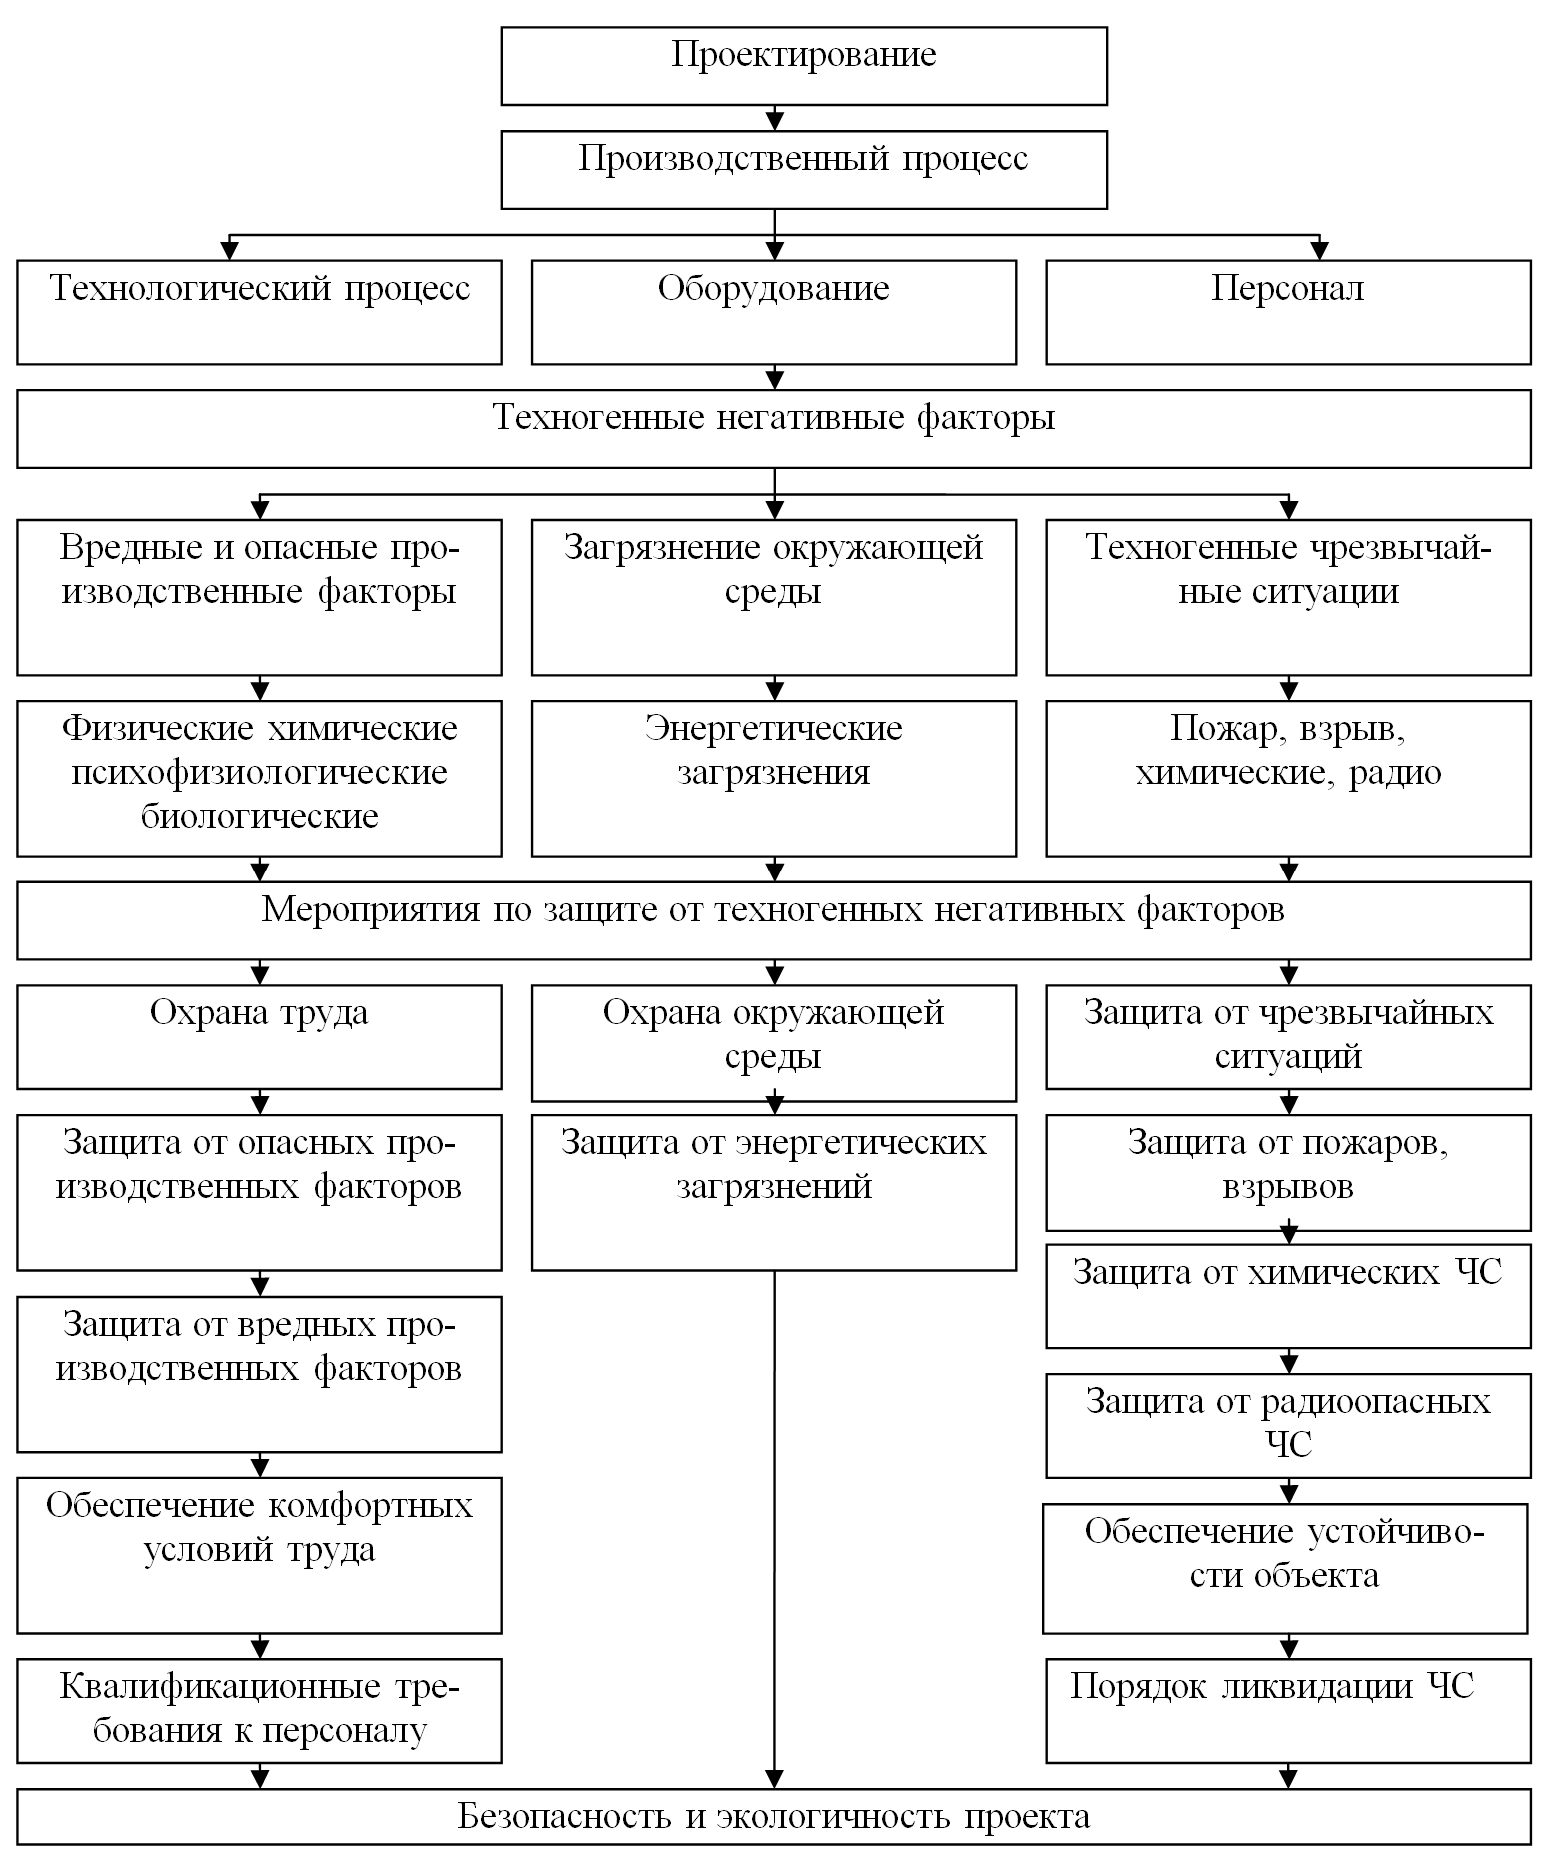
\includegraphics[width=\linewidth]{images/ecology-schema.png}
			\caption{Принципиальная блок-схема обеспечения безопасности объекта проектирования}
			\label{img:ecology-schema}
		\end{minipage}
		\hfill
	\end{center}
\end{figure}  

\subsubsection{Анализ вредных и опасных производственных факторов}

Опасный производственный фактор --- это производственный фактор, воздействие которого в определенных условиях приводит к травме или к другому внезапному ухудшению здоровья. 

Воздействие вредного производственного фактора в определенных условиях приводит к заболеванию или снижению работоспособности.

Опасные и вредные производственные факторы согласно ГОСТ 12.0.003-74 подразделяются по природе действия на следующие группы:

\begin{enumerate}
	\item физические;
	\item химические;
	\item биологические;
	\item психофизические.
\end{enumerate}

Все факторы, за исключением психофизических, обусловлены воздействием техники и рабочей среды.
Психофизиологические факторы связаны с влиянием тяжести и напряженности труда, что в конечном итоге также может привести к заболеваниям.

Так как на рабочем месте, рассматриваемом в рамках данного дипломного проекта, химические и биологические опасные и вредные производственные факторы оказывают незначительное, по сравнению с  физическими факторами, влияние, и в рассмотрение они браться не будут.

При работе с ПЭВМ на пользователя в той или иной степени могут воздействовать следующие физические факторы: повышенные уровни переменного электромагнитного и электростатического полей; повышенный уровень статического электричества; повышенный уровень низкоэнергетического (мягкого) рентгеновского ионизирующего излучения; повышенные уровни ультрафиолетового и инфракрасного излучения; повышенное содержание положительных аэроионов в воздухе рабочей зоны; пониженное содержание отрицательных аэроионов; аномальный уровень освещённости рабочей зоны; повышенная яркость фрагментов светового изображения или света, попадающего в поле зрения пользователя; повышенная неравномерность распределения яркости в поле зрения пользователя; повышенная внешняя освещённость экрана; повышенные пульсации светового потока источников света или светового потока, излучаемого экраном; неблагоприятный для работы спектр излучения источников света; повышенная временная нестабильность изображения; мерцание экрана; изменение яркости свечения экрана; повышенная прямая блескость, вызванная попаданием в поле зрения работающего чрезмерно яркого света различных излучающих объектов; повышенная отражённая блескость, обусловленная наличием зеркальных отражений (бликов), в том числе от экрана; повышенный уровень шума; аномальные температура, влажность и подвижность воздуха рабочей зоны; повышенное значение напряжения в электрической цепи, замыкание которой может произойти через тело человека; пожар.

\textbf{\point Шум}

Шум является общебиологическим раздражителем и в определенных условиях может влиять на все органы и системы организма человека.
Кроме непосредственного воздействия на орган слуха шум влияет на различные отделы головного мозга, изменяя нормальные процессы высшей нервной деятельности.
Шумовые явления обладают свойством аккумуляции: накапливаясь в организме, он все больше и больше угнетает нервную систему.
Шум -- причина преждевременного утомления, ослабления внимания, памяти.

Согласно СанПиН 2.2.2./2.4.1340-03, допустимым уровнем звукового давления при работе на ВДТ и ПЭВМ не должно превышать 60 дБ.

Мероприятия по защите от шума, проводимые в производственном помещении соответствуют ГОСТ 12.1.003-83 и других мероприятий по улучшению шумовой обстановки не требуется.

\textbf{\point Микроклимат}

Микроклимат помещений --- это климат внутренней среды помещений, который определяется действующими на организм человека сочетаниями температуры, влажности и скорости движения воздуха, а также температуры окружающих поверхностей.

Показателями, характеризующими микроклимат в производственном помещении, являются:

\begin{enumerate}
	\item температура воздуха;
	\item относительная влажность воздуха;
	\item скорость движения воздуха;
	\item интенсивность теплового излучения.
\end{enumerate}

Значительное отклонение микроклимата рабочей зоны от оптимального может быть причиной ряда физиологических нарушений в организме работающих, привести к резкому снижению работоспособности и даже к профессиональным заболеваниям.

В помещениях с вычислительной техникой при выполнении работ операторского типа, связанных с нервно-эмоциональным напряжением, по ГОСТ 12.1.005-88 необходимо соблюдать оптимальные величины показателей:

\begin{enumerate}
	\item температура помещения в переходный период $18-22^{\circ}C$, в холодный период $22-24^{\circ}C$, в теплый период $20-24^{\circ}C$;
	\item подвижность воздуха от 0,1 до 0,2 м/с;
	\item влажность воздуха составляет 60--70\%;
	\item воздействие химических веществ отсутствует;
	\item запыленности и загазованности воздуха нет;
	\item выполняются легкие физические работы (1 категория).
\end{enumerate}

Колебания температуры воздуха допускаются до 4\%.

Для создания нормальных условий труда в производственных помещениях обеспечивают нормативные значения параметров микроклимата --- температуры воздуха, относительную влажность и скорость движения, а также интенсивности теплового излучения.

В ГОСТ 12.1.005-88 указаны оптимальные и допустимые показатели микроклимата в производственных помещениях.
Оптимальные показатели распространяются на всю рабочую зону, а допустимые устанавливают раздельно для постоянных и непостоянных рабочих мест в тех случаях, когда по технологическим техническим или экономическим причинам невозможно обеспечить оптимальные нормы.

Мероприятия по обеспечению оптимальных метеоусловий соответствуют \\ ГОСТ 12.1.005-88 и СНиП 2.04.05-86 и других мероприятий по обеспечению микроклимата не требуется.

\textbf{\point Электрический ток}

Опасное и вредное воздействие на людей электрического тока проявляется в виде электротравм и профессиональных заболеваний.
Степень опасного и вредного воздействий на человека электрического тока зависит от:

\begin{enumerate}
	\item рода и величины напряжения и тока; 
	\item частоты электрического тока;
	\item пути прохождения тока через тело человека (наибольшая опасность воз-никает при непосредственном прохождении тока через жизненно важные органы);
	\item продолжительности воздействия на организм человека (с течением времени резко падает сопротивление кожи человека, более вероятным становится поражение сердца, и накапливаются другие отрицательные последствия);
	\item условий внешней среды.
\end{enumerate}

Согласно ГОСТ 12.1.038-82, человек начинает ощущать протекающий через него ток в 0,3 мА (50 Гц), 0,4 мА (400 Гц) и 1 мА (постоянный).
Это пороговый ощутимый ток.
Ток 10 – 15 мА (50 Гц) называется пороговым не отпускающим.
Он вызывает судорожные сокращения мышц руки, в которой зажат проводник.
Ток 25 – 50 мА (50 Гц) приводит к затруднению и даже прекращению дыхания, а при 100 мА ток вызывает остановку или фибрилляцию сердца (хаотические и разновременные сокращения волокон сердечной мышцы, полностью нарушающие ее работу как насоса), прекращение кровообращения и смерть.
При постоянном токе пороговый не отпускающий ток 50 – 70 мА, а фибрилляционный – до 0,3 А.

Существует два вида электротравм:

Электрические удары --- это возбуждение живых тканей организма протекающим через него электрическим током, проявляющееся в непроизвольных судорожных сокращениях различных мышц тела.
В результате электрического удара могут возникнуть или обостриться сердечно-сосудистые заболевания, а также нервные болезни.
Нередко появляется рассеянность, ослабевают память и внимание.

Электрические травмы --- это поражение внешних частей тела человека, к ним относятся: электрический ожог, электрометаллизация кожи и электрические знаки тока.

Причинами смерти от электрического тока могут быть прекращение работы сердца, остановка дыхания и электрический шок.

\textbf{\point Электромагнитное и ионизирующее излучение}

Электромагнитным излучением называется излучение, прямо или косвенно вызывающее ионизацию среды.
Контакт с электромагнитными излучениями представляет серьезную опасность для человека.

Основным источником электромагнитного излучения при работе с ПЭВМ является монитор.
Дисплей излучает электромагнитные поля (ЭМП) в очень широком диапазоне частот (от 3 Гц до 300 мГц), но преобладают следующие два диапазона:

\begin{enumerate}
	\item поля, создаваемые блоком сетевого питания и блоком кадровой развертки дисплея (например, с частотой 50–150 Гц – электромагнитные поля от блока питания, проводов и системы вертикального отклонения и модуляции луча ЭЛТ); основной энергетический спектр этих полей сосредоточен в диапазоне частот до 1 кГц;
	\item поля, создаваемые блоком строчной развертки и блоком сетевого питания ПЭВМ (если он импульсный); основной энергетический спектр этих полей сосредоточен в диапазоне частот от 15 до 100 кГц.
\end{enumerate}

Защита от электромагнитного излучения компьютера приведены в списке ниже.

\begin{enumerate}[1.]
	\item По возможности, стоит приобрести жидкокристаллический монитор, поскольку его излучение значительно меньше, чем у распространённых ЭЛТ мониторов (монитор с электроннолучевой трубкой). 
	\item Системный блок и монитор должен находиться как можно дальше от человека.
	\item Не оставлять компьютер включённым на длительное время, если он не используется, например, использовать <<спящий режим>> для монитора.
	\item В связи с тем, что электромагнитное излучение от стенок монитора намного больше, лучше постараться поставить монитор в угол, так что бы излучение поглощалось стенами. Особое внимание стоит обратить на расстановку мониторов в офисах.
	\item По возможности сократить время работы за компьютером и чаще прерывать работу.
	\item Компьютер должен быть заземлён. Если есть защитный экран, то его тоже следует заземлить, для этого специально предусмотрен провод на конце которого находиться металлическая прищепка (не цепляйте её к системному блоку).
\end{enumerate}

Ионизирующее излучение --- это любое излучение, вызывающее ионизацию среды, т.е. протекание электрических токов в этой среде, в том числе и в организме человека, что часто приводит к разрушению клеток, изменению состава крови, ожогам и другим тяжелым последствиям.

Излучения на расстоянии 40 см от экрана составляют около 0.08 мкР/ч, что не превышает нормы.
И по данному фактору можно отнести работы с персональным компьютером к допустимым по степени вредности. 

Исходя из вышесказанного, условия работы с персональным компьютером удовлетворяют требованиям Р 2.2.013-94 и СанПиН 2.2.2./2.4.1340 03, но необходимы дополнительные меры защиты в виде регламентирования рабочего времени.

\textbf{\point Освещённость}

Правильно спроектированное и выполненное производственное освещение улучшает условия зрительной работы, снижает утомляемость, способствует повышению производительности труда, благотворно влияет на производственную среду, оказывая положительное психологическое воздействие на работающего, повышает безопасность труда и  снижает травматизм.

Недостаточность освещения приводит к напряжению зрения, ослабляет внимание, приводит к наступлению преждевременной утомленности. 
Чрезмерно яркое освещение вызывает ослепление, раздражение и резь в глазах.
Неправильное направление света на рабочем месте может создавать резкие тени, блики, дезориентировать работающего.
Все эти причины могут привести к несчастному случаю или профзаболеваниям, поэтому столь важен правильный расчет освещенности.

Существует три вида освещения --- естественное, искусственное и совмещенное (естественное и искусственное вместе).

Естественное освещение --- освещение помещений дневным светом, проникающим через световые проемы в наружных ограждающих конструкциях помещений.

Естественное освещение характеризуется тем, что меняется в широких пределах в зависимости от времени дня, времени года, характера области и ряда других факторов.

Искусственное освещение применяется при работе в тёмное время суток и днем, когда не удаётся обеспечить нормированные значения коэффициента естественного освещения (пасмурная погода, короткий световой день).

Освещение, при котором недостаточное по нормам естественное освещение дополняется искусственным, называется совмещённым освещением.

Искусственное освещение подразделяется на рабочее, аварийное, эвакуационное, охранное. Рабочее освещение, в свою очередь, может быть общим или комбинированным. Общее --- освещение, при котором светильники размещаются в верхней зоне помещения равномерно или применительно к расположению оборудования. Комбинированное --- освещение, при котором к общему добавляется местное освещение.

Согласно СНиП II-4-79 в помещений вычислительных центров необходимо применить систему комбинированного освещения.

При выполнении работ категории высокой зрительной точности (наименьший размер объекта различения 0,3--0,5мм) величина коэффициента естественного освещения (КЕО) должна быть не ниже 1,5\%, а при зрительной работе средней точности (наименьший размер объекта различения 0,5.1,0 мм) КЕО должен быть не ниже 1,0\%. В качестве источников искусственного освещения обычно используются люминесцентные лампы типа ЛБ или ДРЛ, которые попарно объединяются в светильники, которые должны располагаться над рабочими поверхностями равномерно.

Требования к освещенности в помещениях, где установлены компьютеры, следующие: при выполнении зрительных работ высокой точности общая освещенность должна составлять 300лк, а комбинированная --- 750лк; аналогичные требования при выполнении работ средней точности --- 200 и 300лк соответственно.

Кроме того все поле зрения должно быть освещено достаточно равномерно --- это основное гигиеническое требование. Иными словами, степень освещения помещения и яркость экрана компьютера должны быть примерно одинаковыми, т.к. яркий свет в районе периферийного зрения значительно увеличивает напряженность глаз и, как следствие, приводит к их быстрой утомляемости.

\subsubsection{Анализ воздействия на окружающую среду}

В жизненном цикле компьютерной техники можно выделить три этапа: производство, эксплуатация, утилизация.

Вопросы защиты окружающей среды в процессе производства компьютеров возникли давно и регламентируются сейчас, в частности стандартом ТСО-03 NUTEC, по которому контролируются выбросы токсичных веществ, условия работы и др.
Согласно ТСО-03 произведенное оборудование может быть сертифицировано лишь в том случае, если не только контролируемые параметры самого оборудования соответствуют требованиям этого стандарта, но и технология производства этого оборудования отвечает требованиям стандарта.

Воздействие компьютеров на окружающую среду при эксплуатации регламентировано рядом стандартов.
Выделяют две группы стандартов и рекомендаций: по безопасности и эргономике.

При утилизации старых компьютеров происходит их разработка на фракции: металлы, пластмассы, стекло, провода, штекеры.
Из одной тонны компьютерного лома получают до 200 кг меди, 480 кг железа и нержавеющей стали, 32 кг алюминия, 3 кг серебра, 1 кг золота и 300 г палладия.

Переработку промышленных отходов производят на специальных полигонах, создаваемых в соответствии с требованиями СНиП 2.01.28-85 и предназначенных для централизованного сбора обезвреживания и захоронения токсичных отходов промышленных предприятий, НИИ и учреждений.

\subsubsection{Анализ возможных чрезвычайных ситуаций}

Чрезвычайная ситуация (ЧС) --- это обстановка на определенной территории, сложившаяся в результате аварии, опасного природного явления, катастрофы, стихийного или иного бедствия, которые могут повлечь или повлекли за собой человеческие жертвы, ущерб здоровью людей или окружающей природной среде, значительные материальные потери и нарушение условий жизнедеятельности людей.

ЧС являются многофакторными событиями, которые могут возникать в результате многочисленных причин, в различных условиях и приводить к разнообразным последствиям.

По происхождению ЧС подразделяются на природные, техногенные, антропогенные, военные.

Под техногенной ЧС понимается состояние, при котором в результате возникновения источника техногенной ЧС на объекте, определенной территории или акватории нарушаются нормальные условия жизни и деятельности людей, возникает угроза их жизни и здоровью, наносится ущерб имуществу населения, народному хозяйству и окружающей среде (ГОСТ 22.0.05-94).

Авария --- опасное техногенное происшествие, создающее на объекте, определенной территории или акватории угрозу жизни и здоровью людей и приводящее к разрушению зданий, сооружений, оборудования и транспортных средств, нарушению транспортного или производственного процесса, а также нанесению ущерба окружающей природной среде (ГОСТ 22.0.05-94). Крупная авария, как правило с человеческими жертвами, является катастрофой.

В соответствии с Постановлением Правительства РФ от 21 мая 2007 г. N 304 <<О классификации чрезвычайных ситуаций природного и техногенного характера>> ЧС подразделяются в зависимости от показателей:

\begin{enumerate}
	\item количество людей, пострадавших в ЧС;
	\item количество людей, у которых оказались нарушены условия жизнедеятельности;
	\item размер материального ущерба;
	\item размер ущерба окружающей среде;
	\item размер зоны распространения поражающих факторов.
\end{enumerate}

При идентификации возможных техногенных ЧС, связанных с объектом проектирования, необходимо провести их анализ в зависимости от происхождения, масштаба распространения, вида поражающих факторов.
Так, например, для котельной возможными ЧС являются пожар, взрыв, вызванные воспламенением газа, мазута; разгерметизация систем, работающих под давлением, и воздействие рабочих сред на человека, а аварии в системах электроснабжения приведут к потере их устойчивости.

Существует ряд отраслей производства, которые, в случае возникновения на них аварий, могут создавать наиболее опасные ситуации.
Они относятся к опасным производственным объектам. 

Из анализа промышленных аварий и катастроф следует, что причинами ЧС зачастую являются ошибки при проектировании и недостаточный уровень современных знаний.

Анализ потенциально опасных факторов, связанных с проектируемым объектом, должен явиться основой для обоснования необходимости расчета защиты от наиболее опасного фактора.

К техногенным относят ЧС, происхождение которых связано с техническими объектами, --- пожары, взрывы, аварии на химически опасных объектах, выбросы радиоактивных веществ, обрушение зданий, аварии на системах жизнеобеспечения.

К природным относятся ЧС, связанные с проявлением стихийных сил природы, --- землетрясения, наводнения, извержения вулканов, оползни, сели, ураганы, смерчи, бури, природные пожары и др.

К экологическим ЧС относятся аномальное природное загрязнение атмосферы, разрушение озонового слоя земли, опустынивание земель, засоление почв, кислотные дожди и др.

К биологическим ЧС относятся эпидемии, эпизоотии, эпифитотии.

К социальным ЧС относятся события, происходящие в обществе: межнациональные конфликты, терроризм, грабежи, геноцид, войны и др.

Антропогенные ЧС являются следствием ошибочных действий людей.

Чрезвычайные ситуации классифицируются в зависимости от количества людей, пострадавших в этих ситуациях, людей, у которых оказались нарушены условия жизнедеятельности, от размера материального ущерба, а также границы зон распространения поражающих факторов чрезвычайной ситуации.

Анализ чрезвычайных ситуаций, имевших место в России за последние годы, позволил выделить причины аварийности и травматизма:

\begin{enumerate}
	\item человеческий фактор — 50,1~\%;
	\item оборудование, техника — 18,1~\%;
	\item технология выполнения работ — 7,8~\%;
	\item условия внешней среды — 16,6~\%;
	\item прочие факторы — 7,4~\%.
\end{enumerate}

В настоящее время заметно возрос удельный вес аварий, происходящих из-за неправильных действий обслуживающего технического персонала (более 50~\%). Часто это связано с недостаточностью профессионализма, а также неумением принимать оптимальные решения в сложной критической обстановке в условиях дефицита времени.

% \subsubsection{Обоснование расчетной части}

\subsection{Мероприятия по охране труда}

Охрана труда --- это система сохранения жизни и здоровья работников в процессе трудовой деятельности, включающая в себя правовые, со\-ци\-льно-эк\-но\-ми\-чес\-кие, организационно-технические, санитарно-гигиенические, лечебно-профилак\-ти\-чес\-кие, реабилитационные и иные мероприятия.

Условно охрану труда (ОТ) можно представить совокупностью четырех составляющих:

\begin{enumerate}
	\item правовая охрана труда (ПОТ);
	\item техника безопасности (ТБ);
	\item производственная санитария (ПС);
	\item пожарная безопасность (ПБ).
\end{enumerate}

В соответствии со ст. 210 ТК РФ основными направлениями государственной политики в области охраны труда являются:

\begin{enumerate}
	\item обеспечение приоритета сохранения жизни и здоровья работников;
	\item принятие и реализация федеральных законов и иных нормативных правовых актов Российской Федерации, законов и иных нормативных правовых актов субъектов Российской Федерации в области охраны труда, а также федеральных целевых, ведомственных целевых и территориальных целевых программ улучшения условий и охраны труда;
	\item государственное управление охраной труда;
	\item государственный надзор и контроль за соблюдением государственных нормативных требований охраны труда;
	\item государственная экспертиза условий труда;
	\item установление порядка проведения аттестации рабочих мест по условиям труда и порядка подтверждения соответствия организации работ по охране труда государственным нормативным требованиям охраны труда;
	\item содействие общественному контролю за соблюдением прав и законных интересов работников в области охраны труда;
	\item профилактика несчастных случаев и повреждения здоровья работников;
	\item расследование и учет несчастных случаев на производстве и профессио-нальных заболеваний;
	\item защита законных интересов работников, пострадавших от несчастных случаев на производстве и профессиональных заболеваний, а также членов их семей, на основе обязательного социального страхования работников от несчастных случаев на производстве и профессиональных заболеваний;
	\item установление компенсаций за тяжелую работу и работу с вредными и (или) опасными условиями труда;
	\item координация деятельности в области охраны труда, охраны окружающей природной среды и других видов экономической и социальной деятельности;
	\item распространение передового отечественного и зарубежного опыта работы по улучшению условий и охраны труда;
	\item участие государства в финансировании мероприятий по охране труда;
	\item подготовка специалистов по охране труда и повышение их квалификации;
	\item организация государственной статистической отчетности об условиях труда, а также о производственном травматизме, профессиональной заболеваемости и об их материальных последствиях;
	\item обеспечение функционирования единой информационной системы охраны труда;
	\item международное сотрудничество в области охраны труда;
	\item проведение эффективной налоговой политики, стимулирующей создание безопасных условий труда, разработку и внедрение безопасных техники и технологий, производство средств индивидуальной и коллективной защиты работников;
	\item установление порядка обеспечения работников средствами индивидуальной и коллективной защиты, а также санитарно-бытовыми помещениями и устройствами, лечебно-профилактическими средствами.
\end{enumerate}

Производственные процессы должны быть пожаро- и взрывобезопасными.
Производственные процессы не должны загрязнять окружающую среду (воздух, почву, водоемы) выбросами вредных веществ.

\subsubsection{Мероприятия по обеспечению комфортных условий труда}

В целях предотвращения неблагоприятного влияния на здоровье работников вредных факторов производственной среды и трудового процесса при исполь-зовании ими персональных электронно-вычислительных машин (ПЭВМ) режим их работы рекомендовано устанавливать в зависимости от вида и категории трудовой деятельности.

Виды трудовой деятельности разделяются на три группы: группа А --- работа по считыванию информации с монитора компьютера с предварительным запросом; группа Б --- работа по вводу информации; группа В --- творческая работа в режиме диалога с ПЭВМ. При выполнении в течение рабочей смены работ, относящихся к разным видам трудовой деятельности, за основную работу с ПЭВМ следует принимать такую, которая занимает не менее 50\% времени в течение рабочей смены или рабочего дня.

Для видов трудовой деятельности устанавливаются три категории тяжести и напряженности работы с ПЭВМ, которые определяются: для группы А --- по суммарному числу считываемых знаков за рабочую смену, но не более 60000 знаков за смену; для группы Б --- по суммарному числу считываемых или вводимых знаков за рабочую смену, но не более 40000 знаков за смену; для группы В --- по суммарному времени непосредственной работы с ПЭВМ за рабочую смену, но не более 6 часов за смену.

В зависимости от категории трудовой деятельности и уровня нагрузки за рабочую смену при работе с ПЭВМ устанавливается суммарное время регламентированных перерывов.

Для предупреждения преждевременной утомляемости пользователей ПЭВМ рекомендуется организовывать рабочую смену путем чередования работ с использованием ПЭВМ и без него.

При возникновении у работающих с ПЭВМ зрительного дискомфорта и других неблагоприятных субъективных ощущений, несмотря на соблюдение санитарно-гигиенических и эргономических требований, рекомендуется применять индивидуальный подход с ограничением времени работы с ПЭВМ.

В случаях, когда характер работы требует постоянного взаимодействия с монитором компьютера (набор текстов или ввод данных и т.п.) с напряжением внимания и сосредоточенности, при исключении возможности периодического переключения на другие виды трудовой деятельности, не связанные с ПЭВМ, рекомендуется организация перерывов на 10 - 15 мин. через каждые 45 - 60 мин. работы.

Продолжительность непрерывной работы с ПК без регламентированного перерыва не должна превышать одного часа.

При работе с ПЭВМ в ночную смену (с 22 до 6 часов) независимо от категории и вида трудовой деятельности продолжительность регламентированных перерывов следует увеличивать на 30 \%.

Существует множество превентивных (предупредительных) мероприятий, позволяющих повысить безопасность работы.
Одно из них заключается в создании на рабочем месте соответствующего инженерного обеспечения.
Задача --- сделать работу более комфортабельной, менее утомительной, помочь работнику стать более бдительным, менее открытым для несчастных случаев.

Работающим на ПЭВМ с высоким уровнем напряженности во время регламентированных перерывов и в конце рабочего дня рекомендуется посещать специально оборудованные комнаты для снятия напряжения.

\subsubsection{Мероприятия по защите от опасных и вредных производственных факторов}

Задачей защиты человека от опасных вредных производственных факторов (ОВПФ) является снижение уровня вредных факторов, не превышающих ПДУ и ПДК и риска появления опасных факторов до величин приемлемого риска.

Основные мероприятия по защите человека от опасных и вредных производственных факторов приведены ниже.

\begin{enumerate}[1.]
	\item Совершенствование технологии производств и технических средств с целью снижения уровня ОВПФ.
	\item Защита расстоянием (удаление от источника ОВПФ).
	\item Защита временем (уменьшение времени пребывания в зоне действия \\ ОВПФ).
	\item Применение средств защиты:
	\begin{enumerate}
		\item применение средств коллективной защиты;
		\item применение средств индивидуальной защиты.
	\end{enumerate}
\end{enumerate}

Защита человека от физических негативных факторов осуществляется тремя основными методами:

\begin{enumerate}
	\item ограничение времени пребывания в зоне действия физического поля;
	\item удаление от источника поля;
	\item применение средств защиты.
\end{enumerate}

Для защиты от акустических колебаний (шума, ультра и инфразвука) проводят следующие мероприятия:

\begin{enumerate}
	\item снижение звуковой мощности источника звука;
	\item размещение рабочих мест с учетом направленности излучения от источника звука;
	\item акустическая обработка помещений (применение звукопоглощения облицовки, штучные, объемные поглотители различных конструкций, подвешенные к потолку помещений);
	\item применение звукоизоляции (глушители);
	\item применение средств индивидуальной защиты (наушники, шлемы, беруши).
\end{enumerate}

Для снижения воздействия электромагнитного и ионизирующего излучения рекомендуется применять мониторы с пониженным уровнем излучения, устанавливать защитные экраны, а также соблюдать регламентированные режимы труда и отдыха.

Защита работника от негативного воздействия источника внешнего ионизирующего излучения достигается путем:

\begin{enumerate}
	\item снижение мощности источника излучения до минимально необходимой величины;
	\item увеличение расстояния между источником излучения и работником;
	\item уменьшение продолжительности работы в зоне излучения;
	\item установление между источником излучения и работником защитного экрана.
\end{enumerate}

%\subsubsection{Мероприятия по защите от вредных производственных факторов}
%\subsubsection{Квалификационные требования к персоналу}

\subsection{Мероприятия по охране окружающей среды}

Для охраны окружающей среды необходимо разработать и освоить оптимальную технологию утилизации устаревших или пришедших в негодность внутренних заменяемых компонентов компьютера (интегральных схем, плат, микроконтроллеров, механических частей компьютера, шлейфов и~т.д.), а также внешних магнитных носителей.

Для этого на первом этапе утилизации необходимо сортировать и складировать в отдельные контейнеры отходы <<различной природы>> (отдельно провода, отдельно платы, отдельно различные механизмы, отдельно бумагу).

На втором этапе нужно отделять от неработающих деталей исправные части и использовать их в качестве запчастей для работающих изделий, если это возможно.

Оставшиеся --- сдавать в соответствующие профильные ремонтные или утилизирующие организации.

\subsection{Мероприятия по защите от чрезвычайных ситуаций}

В качестве основных направлений в решении задач обеспечения защиты от чрезвычайных ситуаций могут рассматриваться следующие:

\begin{enumerate}
	\item прогнозирование и оценка возможных последствий чрезвычайных ситуаций;
	\item планирование мероприятий по предотвращению или уменьшению вероятности возникновения чрезвычайных ситуаций, а также сокращению масштабов их последствий;
	\item обеспечение устойчивой работы объектов народного хозяйства в чрезвычайных ситуациях;
	\item обучение населения действиям в чрезвычайных ситуациях;
	\item ликвидация последствий чрезвычайных ситуаций.
\end{enumerate}

Для тушения пожаров в рассматриваемом помещении нужно использовать либо порошковые составы, либо установки углекислотного тушения, т.к. при использовании воды и пены велика вероятность поражения электрическим током.

Выбор типа огнетушителя (передвижной или ручной) обусловлен размерами возможных очагов пожара. При их значительных размерах необходимо использовать передвижные огнетушители.

Число огнетушителей одного из типов для разных категорий помещений необходимо устанавливать из таблиц, приведенных в нормах оснащения помещений ручными или передвижными огнетушителями.

Расстояние от возможного очага пожара до места размещения огнетушителя не должно превышать 30 м для помещений категории В и 70 м для помещений категории Д.

Огнетушители должны всегда содержаться в исправном состоянии, периодически осматриваться, проверяться и своевременно перезаряжаться.

Для профилактики пожарной безопасности организуется обязательный инструктаж по правилам пожарной безопасности. Кроме этого необходимо наличие планов эвакуации и назначение ответственных лиц.

Рассматриваемое рабочее место оборудовано огнетушителем и системой пожарной сигнализации.

Дополнительных мер по защите от ЧС не требуется.

\subsection{Расчётная часть}

\subsubsection{Расчёт освещённости}

Профессиональным заболеванием операторов и программистов является ухудшение зрения.
Так как параметры помещения, в котором ведется работа, и используемой техники (персональной ПЭВМ) удовлетворяют санитарным нормам, то особое внимание следует уделить освещенности рабочего места.

Расчет освещенности проводится с путем расчета коэффициента использования с использованием метода светового потока).
Он позволяет учесть прямую и отраженную составляющую светового потока от потолка, стен и рабочих поверхностей.

Имеются следующие исходные данные:
\begin{enumerate}
  \item площадь помещения --- 2,5x4 м;
  \item высота подвеса светильников $h_\textup{св}$= 2,5 м;
  \item источник освещения --- лампа люминесцентная (ЛБА), яркость фона --- светлая;
  \item яркость объекта --- средняя;
  \item система освещения --- общая;
  \item коэффициент отражения побеленного потолка: $p_\textup{п}$= 0,7;
  \item коэффициент отражения стен, обклеенных обоями: $p_c$ = 0,5;
  \item коэффициент отражения расчетной поверхности: $p_p$ = 0,3.
\end{enumerate}

По таблице <<Нормы освещенности при искусственном освещении и коэффициент естественного освещения (для 3 пояса светового климата РФ) при естественном и совмещенном освещении>> (СНиП 23-05-95), исходя из характеристик зрительной работы определяем разряд и подразряд зрительной работы как IV-В.
Данному разряду соответствует норма искусственного освещения при системе комбинированного освещения 300 лк.

Норма рабочего искусственного освещения составляет $E_\textup{он}$ = 400 лк. Коэффициент запаса равен $K_3$ = 1,5, высота подвеса светильников $h_\textup{св}$ = 2,2 м.

Определяем индекс помещения:

$i = {{a \cdot b} \over {(a + b) \cdot h_\textup{св}}} = {{2,5 \cdot 4} \over {(2,5 + 4) \cdot 2.5}} {\approx 0,6}$

Тип лампы --- ЛБА, люминесцентная белого света, амальгамная.
Интерполированием находим коэффициент использования: $\eta$ = 0,52.

Определяем расстояние между светильниками и по нему --- число светильников в помещении.
Рекомендованное отношение $\lambda = \frac{I_\textup{св}}{h_\textup{св}}$ равно 0,8--1,2. Принимаем $\lambda$ = 0,8, тогда  $I_\textup{св} = 0,8 \cdot 2,5 = 2$ м.

Число светильников при размещении по углам квадрата вычисляется по формуле:

$n = {{a \cdot b} \over {I_\textup{св}^2}} = {{2,5 \cdot 4} \over {4}} \approx 3$

Определяем световой поток одной лампы.
Коэффициент минимальной освещенности, зависящий от размещения и светораспределения светильников, создающих некоторую неравномерность распределения светового потока по расчетной плоскости, принимаем равным $Z$ = 1,1.

$\Phi_o = {{E \cdot S \cdot Z \cdot K_3} \over {n \cdot \eta}} = {{400 \cdot 10 \cdot 1,1 \cdot 1,5} \over {3 \cdot 0,52}} \approx 4231 (\textup{лм})$

Выбираем лампу ЛБ-80-7 со световым потоком 5200 лм, срок продолжительности горения 12000 час, мощность 80 Вт.
Суммарная мощность осветительной установки общего освещения:

$P = P_o \cdot n = 80 \cdot 3 = 240 (\textup{Вт})$

Таким образом, на площадь 2,5 x 4 м для работы за дисплеем при общем освещении должны использоваться 3 светильника по 1 лампе ЛБА-80-7.

\subsubsection{Расчёт освещённости}

Одним из неблагоприятных факторов производственной среды является высокий уровень шума, создаваемый печатными устройствами, оборудованием для кондиционирования воздуха, вентиляторами систем охлаждения в самих ЭВМ.

Для решения вопросов о необходимости и целесообразности снижения шума необходимо знать уровни шума на рабочем месте оператора.

Уровень шума, возникающий от нескольких некогерентных источников, работающих одновременно, подсчитывается на основании принципа энергетического суммирования излучений отдельных источников:

\begin{equation}
	L_{\sum}=10 lg \sum^{i=n}_{i=1} 10^{0.1L},
\end{equation}
\begin{ESKDexplanation}
	\item где $L_i$ --- уровень звукового давления i-го источника шума;
	\item $n$ --- количество источников шума.
\end{ESKDexplanation}

Полученные результаты расчета сравнивается с допустимым значением уровня шума для данного рабочего места.
Если результаты расчета выше допустимого значения уровня шума, то необходимы специальные меры по снижению шума.
К ним относятся: облицовка стен и потолка зала звукопоглощающими материалами, снижение шума в источнике, правильная планировка оборудования и рациональная организация рабочего места оператора.

Уровни звукового давления источников шума, действующих на оператора на его рабочем месте представлены в табл.~\ref{tab:ecol-noisesource}.

\begin{footnotesize}
\begin{longtable}[h]{|p{0.45\textwidth}|p{0.45\textwidth}|}
	\caption{\label{tab:ecol-noisesource}Уровни звукового давления различных источников} \\
	\hline
		\textbf{Источник шума} & \textbf{Уровень шума, дБ} \\
	\hline \endhead
		Жесткий диск & 40 \\
	\hline
		Вентилятор & 45 \\
	\hline
		Монитор & 17 \\
	\hline
		Клавиатура & 10 \\
	\hline
		Принтер & 45 \\
	\hline
		Сканер & 42 \\
	\hline
\end{longtable}
\end{footnotesize}

Обычно рабочее место оператора оснащено следующим оборудованием: винчестер в системном блоке, вентилятор(ы) систем охлаждения ПЭВМ, монитор, клавиатура, принтер и сканер.

Подставив значения уровня звукового давления для каждого вида оборудования в формулу, получим:
$L_{\sum}=10 lg (10^4 + 10^{4.5} + 10^{1,7} + 10^1 + 10^{4.5} + 10^{4.2}) = 49.5$ дБ.

Полученное значение не превышает допустимый уровень шума для рабочего места оператора, равный 65 дБ (ГОСТ 12.1.003-83).
И если учесть, что вряд ли такие периферийные устройства как сканер и принтер будут использоваться одновременно, то это число будет еще ниже. 

\subsection{Оценка эффективности принятых решений}

В данном разделе был произведен анализ основных вредных и опасных факторов исследуемого объекта.
По результатам анализа были разработаны мероприятия по обеспечению безопасных и комфортных условияй труда оператора ЭВМ.

Для проверки соответствия рабочий условий нормативным был произведен расчет освещенности.

Были разработаны мероприятия по охране окружающей среды и противостоянию возможным чрезвычайным ситуациям.

На основании выше изложенного, при условии выполнения всех мероприятий, соблюдения норм трудовой дисциплины и распорядка дня, рабочее место оператора персональной ЭВМ можно считать соответствующим классу труда 3.1.

Такие условия труда характеризуются такими отклонениями уровней вредных факторов от гигиенических нормативов, которые вызывают функциональные изменения, восстанавливающиеся, как правило, при более длительном (чем к началу следующей смены) прерывании контакта с вредными факторами и увеличивают риск повреждения здоровья.

\clearpage
\newpage
